\section{Approach} \label{sec:apprach}

The main concept in Squirrel is the \textit{resource-aware container}.
Such containers are logical entities that take care of the resource management concern.
By logical we mean that it is not important, from a functional point of view, how a
container achieves resource management. 
Instead, a resource-aware container is an entity that \textit{wraps} a set of components and offers the following properties:
\begin{itemize}
\item \textbf{Resource consumption monitoring} refers to the ability to assess the 
quantity of resources used by a component.
\item \textbf{Resource reservation} is the capacity to ensure a given amount of
resources will be available whenever a component demands it.
\item \textbf{Resource isolation} guarantees that a component's behavior in terms
of resource usage does not interfere with the behavior of another component.
\end{itemize} 

%Even the idea of 
\textit{Wrapping} a set of components can be considered a soft definition because the \textit{membrane} of a resource-aware container limits the behavior
of the contained components only when it is relevant to the resource management concern.
For instance, components within different containers can still communicate directly
with each other through their interfaces without intervention of their containers as long as such communication does not affect the resource under management.  

In Squirrel we propose to automatically select, deploy and configure resource containers to manage resource usage.
The novelty is that we delay the selection of the container's implementation till deployment-time in order to have knowledge about the exact conditions of the system and thus minimize the overhead of the resource management system.
This idea is supported by the claim that components often require disjoint sets of resource types.
Our framework is composed of three essential elements: i) a mechanism to describe the management requirements of an application, ii) an admission control scheme in the middleware to handle the global view of resource availability, and iii) mechanisms to map component model concepts to system-level abstractions.
In the following subsections we describe our framework and its elements.

\subsection{Managing resources through architecture adaptations}
Modern application development models, such as component-based systems, promote the usage of Architecture Description Languages (ADL) or configuration models to check properties on the system's structure and to drive system deployment. 
In Squirrel, we propose to enhance this layer with metadata regarding resource reservation and to use these metadata to efficiently drive resource reservation offered at the system level.  
The idea is to follow a gray-box approach where we automatically adapt a component-based application by applying an architecture pattern to isolate a component within a resource-aware container.

\begin{figure}[htbp]
\centering
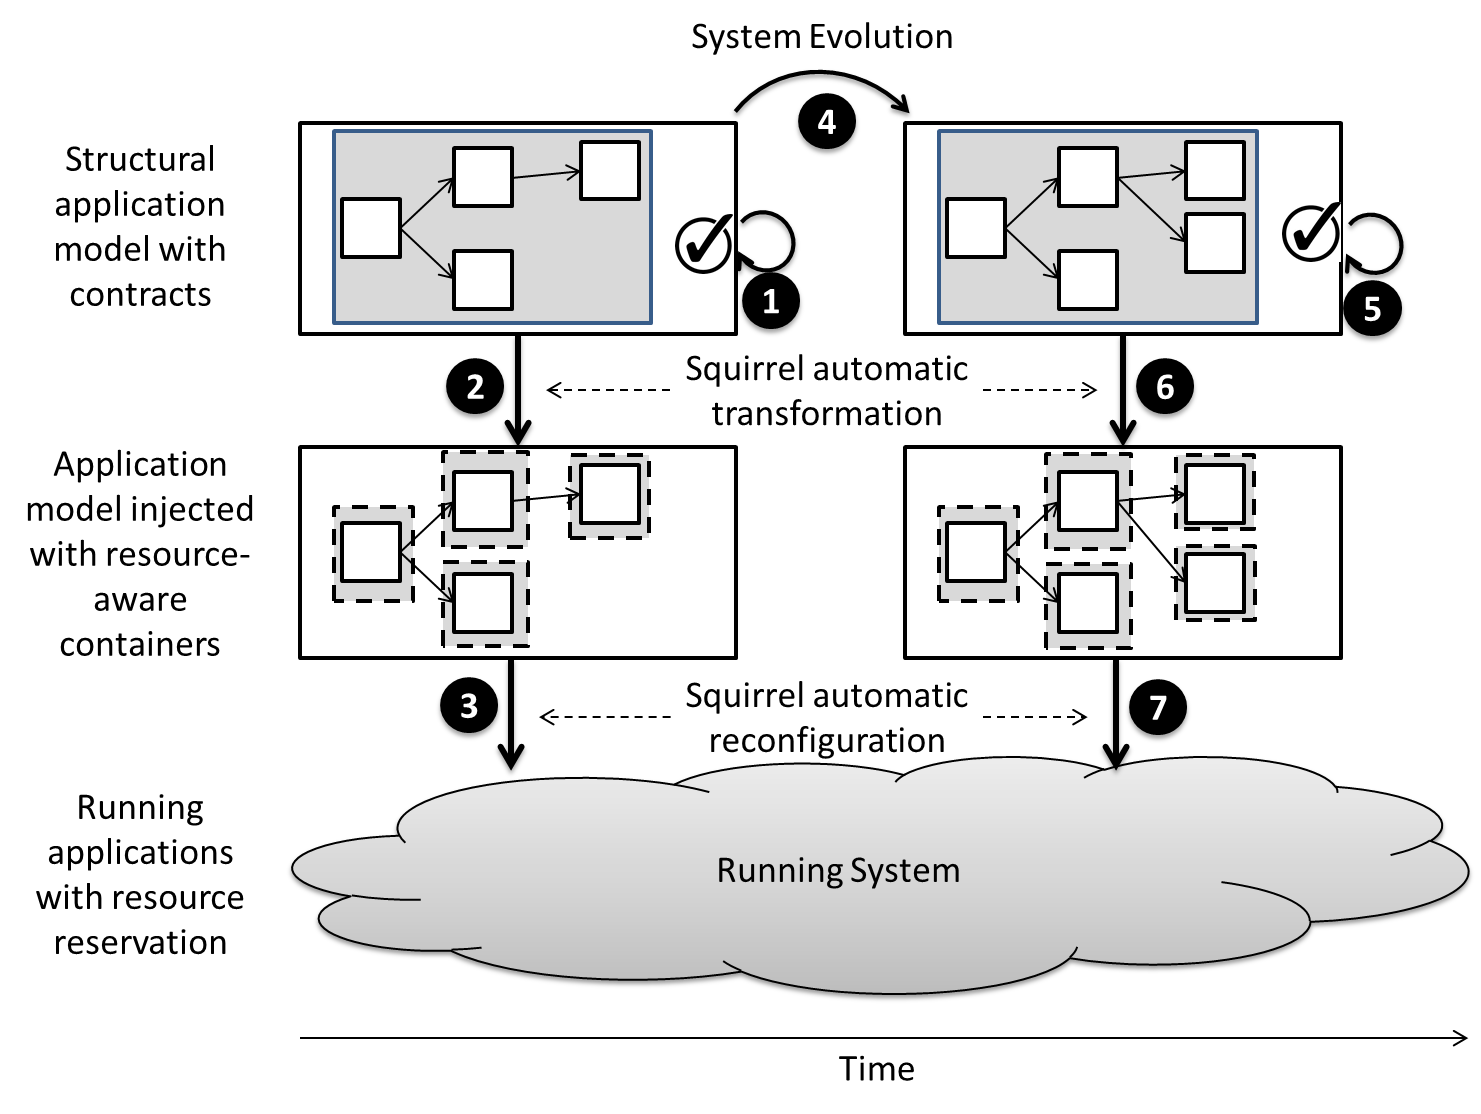
\includegraphics[width=0.7\textwidth]{chapter4/figures/globalOverview.png}
\caption{Squirrel approach for resources reservation} \label{fig:Overview}
\vspace{-0.5cm}
\end{figure}	

As illustrated in figure~\ref{fig:Overview}, Squirrel follows an automatic process to manage resources.
Squirrel receives an application's model, enhanced with contracts on resource reservation. 
Squirrel performs admission control to check the validity of the contracts on resource usage with respect to the available resources in the execution environment.
If the contracts are consistent with available resources, the process continues, if not, the application's model is refused.
Then, as depicted by arrow 2, Squirrel automatically transforms components or the configuration/architecture model by isolating components in resource-aware containers that can be finely configured to decrease the resource management overhead.
Finally, as depicted by arrow 3, Squirrel reconfigures the running system.
When the application evolves (arrow 4), 
%Squirrel automatically adapts the system while preserving resource reservation properties by applying the whole process on the new model (arrow 5, 6 and 7).
Squirrel attempts to preserve resource reservation properties while processing the new model (arrow 5, 6 and 7).


\subsection{Describing resource management requirements}
Beugnard et al. discuss the extending Meyer's \textit{Design-By-Contract} idea to software components~\cite{Beugnard774917}.
They classify component contracts into four categories: syntactic (level 1), semantic (level 2), synchronization (level 3), and Quality of Service (level 4).
%They explain that component contracts have to deal with concerns that they classified into 
%Fifteen years later, many component-based frameworks provide contracts that are used to: 
%i) Describe the component features with all required contracts.
%ii) Select from all contracts those that are useful in the context of component use, and configure them.
%iii) Evaluate contracts and react accordingly.
%iv) Decide when to stop evaluating contracts. 
There is no de-facto standard to describe component contracts, but many domain specific interface description languages contain such metadata.
This chapter assumes that components have contracts to deal with resource reservation (level 4).
A contract in Squirrel defines component resource requirements written in terms of resource types, quotas and expected component usage.
\begin{itemize}
\item{\textbf{Definition 1}} A resource type indicates any class of computational resource that is useful to a component.
Its consumption must be susceptible to monitoring and reservation.
In this chapter, we consider CPU, Memory, Network Bandwidth and IO Throughput.

\item{\textbf{Definition 2}} Expected component usage describes the expected number of external invocations of each method of the component interface.
In short, let $C$ be a component instance, then $\forall{I \in C_{Interfaces}}, \forall{M \in I_{methods}} \\ {EU}_{IM}$ is the number of expected invocations of method $M$, per second.

\end{itemize}

A \textbf{contract in Squirrel} is a set of tuples with the form $\langle RT, N, MU \rangle$ where $RT$ is a resource type, N the maximum amount of resources to reserve, and $MU$ is the measuring unit used for this resource type.
Optionally, Squirrel supports the definition of a set of tuples with the form $\langle I, M, {EU}_{IM} \rangle$ where $I$ is a component interface, $M$ is a method of the interface, and ${EU}_{IM}$ the expected usage.
Implementations of the Squirrel approach must provide a way to define contracts with these concepts.
%In section~\ref{sec:kevoree} 
We use a domain-specific language to describe contracts.

\subsection{Admission control} \label{sect:admissionControl}

Providing resource reservation in a component based framework requires checking if components' resource-aware contracts are compatible with the resources available in the execution environment.
%The platform provides a fixed amount of resources that constitute the pool of resources used by components.
By checking the availability of resources, the platform controls component admissions.

%To support this dynamism while managing resources, 
To support resource management at runtime, Squirrel takes into account two events: i) component deployment, and ii) component removal.
%These are common operations on any middleware; hence adding a notification for these events is straightforward.
Whenever the application is modified, the system automatically recalculates the aggregated resources required by the application and compares it to the available resources in the execution environment.
If the available resources are greater than those required by the application, the reconfiguration is accepted, else, the application model is refused and the reconfigurations are discarded.

%\subsection{Defining multiple variants of execution model}
%\todo{I couldn't finish this, so I'm writing my ideas}
%To support our approach, a middleware needs to support multiple ways of mapping component instances into system/runtime abstractions.
%Somehow, it means that it needs an extension point to describe a factory for creating component instances.
%I can see two ways of doing so, either the writer of the middleware provides many versions of execution model or she provides a mechanism to extends the semantic of a component instance and of component containers (Node).
%In Kevoree we achieved this easily because it is naturally extensible, we can define new Node Types, New Channel Type, and we can compose them.
%Moreover, we use Models@Runtime to easily change between variant of mappings (e.g., we receive a model where each component is executed as a Thread and sometime we transform the model in order to execute components as processes). 

\subsection{Mapping component-model concepts to system-level abstractions}

%To map component-model concepts to system-level abstractions that allow for resource management, Squirrel defines steps to perform either during the design/implementation of the platform or at deployment time.
Squirrel defines steps to map component-model concepts to system-level abstractions that allow for resource management. Mappings can be applied during the design and implementation of the framework, or at deployment-time.
During framework design/implementation, developers identify system abstractions that are suitable to represent each concept and implement the respective mappings.
As a second step, resource management methods for each abstraction are implemented and evaluated.
This evaluation is used to determine the management methods with lowest overhead for each pair of system abstraction and resource type.
Later on, at deployment-time, the platform selects a component-to-system mapping using optimization techniques and the data obtained at design-time.
In this section, we briefly explain each step.

As we have mentioned, components can be represented through different system abstractions. % in the runtime platform.
This requires \textit{identifying possible mappings from components to system-level abstractions}.
Mappings must respect the semantics of the component model, and %but for a resource-aware platform, 
must provide resource management capabilities.
A key problem is that different mappings have different non-functional properties, and optimizations are often needed to make the mappings attractive. % competitive.
Additionally, an extensible design of the component platform, where it is easy to accommodate new mappings, greatly facilitates the co-existence of different mappings to represent a component. 
The set $ \textit{SA} $ of system abstractions that are available to represent a concept, along with the recommended optimizations for each abstraction, are defined in this step.

During the design/implementation of the platform it is necessary to \textit{define methods to manage resources} for each pair of system abstraction and resource type.
Developers must devise resource management methods for each mapping
% and resource type, 
 and identify the least costly.
If we consider different abstractions and resource types, we can define the matrices $ M $ and $ C $ where
$ \forall{\textit{sa} \in \textit{SA}, \textit{rt} \in \textit{RT}} $ the values
$  M_{\textit{sa}, \textit{rt}} $ and $ C_{\textit{sa}, \textit{rt}} $ indicate the method that minimizes the cost of managing the resource $ \textit{rt} $ when the abstraction $ \textit{sa} $ is used to represent a component. %, and this minimum cost.
%\hl{In a simple setting, the cost of each pair could be calculated as the mean overhead produced by the management method when some benchmarks are executed.[IS THIS PHRASE NECESSARY?]}
We make two assumptions about the resource management mechanisms: i) mechanisms are always composable if they manage different resource types, and ii) the costs of any pair of management mechanisms are independent.

At deployment-time, \textit{the platform selects the mapping} to use for each component in the application. % to deploy.
To do so, the platform uses the information contained in the matrices $ M $ and $ C $, the set of possible optimizations for each mapping, and the resource requirements of the application.
At this stage, the only data needed regarding resource requirements is the type of resource.
%Using this data, it is possible to apply an optimization method to select the best mapping candidate.
Using this data allows selecting the best mapping candidate.
Although we only use a single cost matrix that contains the overhead of each management mechanism, we think it is easy to generalize the approach to handle multi-objective optimizations with more than one cost matrix.
Others refinement to evaluate the cost of a mapping are possible.
For instance, we can consider the cost of using a specific binding to connect two components that use a given mapping.
Finally, there are many optimization methods that can compute the mappings, we do not propose any particular method in the approach.
However, the results shown in section~\ref{sec:evaluation} suggest that very simple heuristics can lead to good performance. 
 

%\todo{Here we should talk about the heuristic. We are trying to optimize, so we need to choose a mapping for each component. We only have a partial information about each resource managment mechanism. that's why we cannot perform classic optimization and we relies on heuristics}
%\todo{A conclusion here}
